% !Mode:: "TeX:UTF-8"
%%==========================
%% chapter01.tex for SJTU Master Thesis
%% based on CASthesis
%% modified by wei.jianwen@gmail.com
%% version: 0.3a
%% Encoding: UTF-8
%% last update: Dec 5th, 2010
%%==================================================

%\bibliographystyle{sjtu2} %[此处用于每章都生产参考文献]
\chapter{实验结果}
\label{chap:exp}
\section{数据集}
我们在两个数据集上进行了评测,一个是Buffy数据集,一个是DL(daily life)数据集。
Buffy数据集包含了748张从Buffy TV秀中截取下来的图片,每张图片包含了人体各个部位的位置标签。
这个数据集是人体姿势预测问题的标准数据集,很多已有的工作都是在这个上面进行的。
DL数据集包含了997张人体生活照片,是我们从Flickr图片社交分享网站上抓取下来的。
我们对他进行了手工标注,标注了人体各个部位的位置标签。
跟Buffy数据集相比,DL数据集拥有更丰富的衣服属性信息。
为了对我们求解的衣服属性值进行评测,我们手动为Buffy和DL标注了衣服属性标签信息。
为了训练和评测,我们对每个数据集进行了切分。
对于Buffy数据集,选取472张图片作为训练数据集,剩下的作为测试数据集。
对于DL数据集,我们选取200张图片作为训练数据集,剩下的作为测试数据集。

\begin{table}
\centering
\caption{在Buffy数据集上和前人工作的对比}
\begin{tabular}{|c|c|c|c|c|c|} \hline
    Method & Torse & Upper arms & Lower arms & Head & Total \\ \hline
Andriluka et al.~\cite{cvpr09} &  90.7 & 79.3 & 41.2 & 95.5 & 73.5 \\ \hline
Sapp et al.~\cite{eccv10} & \textbf{100} & 95.3 & 63.0 & 96.2 & 85.5 \\ \hline
Yang and Ramanan~\cite{deva11} & \textbf{100} & 96.6 & 70.9 & \textbf{99.6} & 89.1 \\ \hline
Our Approach & \textbf{100} & \textbf{97.1} & \textbf{78.4} & 99.1 & \textbf{91.6} \\ \hline
\end{tabular}
\label{tb:buffy}
\end{table}

\begin{table}
\centering
\caption{在DL数据集上和前人工作的对比}
\begin{tabular}{|c|c|c|c|c|c|} \hline
    Method & Torse & Upper arms & Lower arms & Head & Total \\ \hline
Andriluka et al.~\cite{cvpr09} &  97.0 & 91.7 & 84.5 & 94.0 & 90.6 \\ \hline
Sapp et al.~\cite{eccv10} & \textbf{100} & 88.5 & 78.0 & 87.6 & 86.8 \\ \hline
Yang and Ramanan~\cite{deva11} & 99.8 & 95.7 & 87.5 & 95.6 & 93.6 \\ \hline
Our Approach & \textbf{100} & \textbf{97.2} & \textbf{91.3} & \textbf{99.1} & \textbf{95.7} \\ \hline
\end{tabular}
\label{tb:dl}
\end{table}

\section{实验评测规则}
我们和已有的三份工作进行了对比,包括Andriluka等\cite{cvpr09},Sapp等\cite{eccv10},Yang and Ramanan等\cite{deva11}。
对于人体姿势预测的结果,我们采用标准的评测指标,即就是正确姿势的概率PCP\cite{fer09},它代表了正确的姿势所占的比例。
对于衣服属性的聚类结果,我们采用聚类工作中的标准指标F1分值来进行评测。
我们用$K$-Means聚类的结果作为衣服属性的基准,对于已有的三份工作,我们用他们得到的姿势解来求得最优的衣服属性,然后进行$K$-Means聚类。


\begin{figure}[tbp]
\centering
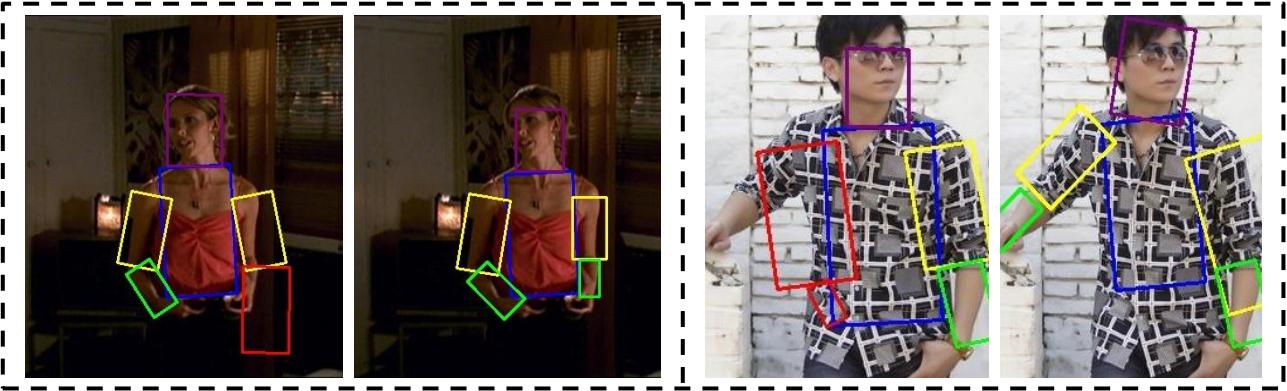
\includegraphics[width=0.9\textwidth]{img/compare.jpg}
\bicaption{\textbf{我们的方法和 Yang and Ramanan~\cite{deva11}的对比 }
第1和3个结果是Yang and Ramanan~\cite{deva11}的方法产生的,我们发现这在上臂和下臂上得到了错误的结果。
而我们的方法(第2和4个)得到了正确的结果。}{\textbf{我们的方法和 Yang and Ramanan~\cite{deva11}的对比 }
第1和3个结果是Yang and Ramanan~\cite{deva11}的方法产生的,我们发现这在上臂和下臂上得到了错误的结果。
而我们的方法(第2和4个)得到了正确的结果。}{Fig}{\textbf{Comparison of our approach with Yang and Ramanan~\cite{deva11} }
Yang and Ramanan~\cite{deva11} produces incorrect estimation (the 1st and 3rd) for upper and lower arms,
while our latent clothing attribute approach produces correct.}
\label{fig:compare}
\end{figure}

\section{实验结果分析}
图6展示了我们算法得出的一些结果,可以定性的看出,我们的算法取得了不错的效果。
在表2和表3中我们分别展示了Buffy和DL数据集的PCP评测结果。
对于Buffy数据集,表2显示我们的方法超越了目前最好的方法Yang and Ramanan\cite{deva11}。
众所周知,下臂的检测是最具有挑战性的,但是令人惊喜的是,我们的方法比目前最好的方法超过了7.5个百分点,这是一个很大的提升了,显示了我们将衣服属性考虑进去的优越性。
对于DL数据集来说,我们的方法超越了目前已有的所有方法。

我们的方法附加的产出是对具有相似衣服属性的图片进行了聚类,图5分别展示了Buffy和DL数据集上的结果。
在图5的上半部分中,我们展示了Buffy数据集的聚类效果,DL数据集的聚类效果在下方。
表4和表5显示了每一种方法的F1分值,可以看出,我们的方法极大的提高了聚类的准确性,比基准要高出很多。
这很大程度上是因为我们的模型训练策略和迭代式的优化算法。
注意到,“$K$-Means+Groundtruth“为我们的模型训练提供了初始的衣服属性标签信息,这也验证了我们方法的有效性。

\begin{table}
\centering
\caption{在Buffy数据集上对衣服属性结果的F1分值}
\begin{tabular}{|c|c|c|c|c|} \hline
    HPE & Sleeve & Neckline & Pattern & Total \\ \hline
Andriluka et al.~\cite{cvpr09} + $K$-Means & 24.1 & 26.6 & 34.2 & 28.3  \\ \hline
Sapp et al.~\cite{eccv10} + $K$-Means & 22.9 & 27.9 & 40.5 & 30.4 \\ \hline
Yang and Ramanan~\cite{deva11} + $K$-Means & 38.3 & 25.7 & 22.6 & 28.9\\ \hline
Groundtruth + $K$-Means & 34.7 & 36.1 & 39.5 & 36.8\\ \hline
Our Approach & \textbf{55.6} & \textbf{68.8} & \textbf{80.8} & \textbf{68.4}  \\ \hline
\end{tabular}
\label{tb:f1_buffy}
\end{table}


\begin{table}
\centering
\caption{在DL数据集上对衣服属性结果的F1分值}
\begin{tabular}{|c|c|c|c|c|} \hline
    HPE & Sleeve & Neckline & Pattern & Total \\ \hline
Andriluka et al.~\cite{cvpr09} + $K$-Means & 27.5 & 31.7 & 27.6 & 28.9  \\ \hline
Sapp et al.~\cite{eccv10} + $K$-Means & 34.9 & 30.5 & 23.8 & 29.7 \\ \hline
Yang and Ramanan~\cite{deva11} + $K$-Means & 43.2 & 28.6 & 35.8 & 35.9 \\ \hline
Groundtruth  + $K$-Means & 31 & 29.8 & 26.1 & 28.9 \\ \hline
Our Approach & \textbf{57.2} & \textbf{60.3} & \textbf{74.7} & \textbf{64.1}  \\ \hline
\end{tabular}
\label{tb:f1_dl}
\end{table}


\begin{figure*}[tbp]
\centering
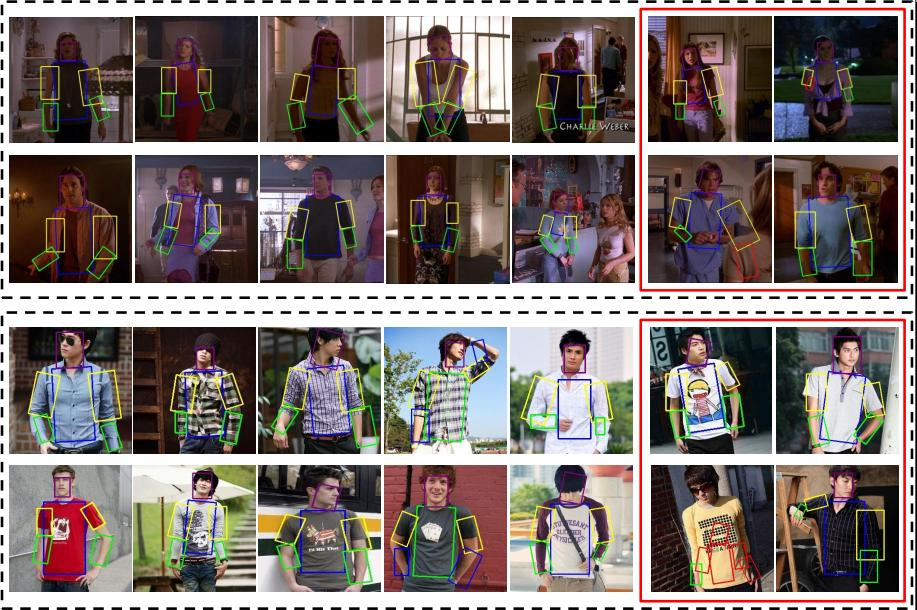
\includegraphics[width=\textwidth]{img/attr.jpg}
\bicaption{\textbf{Buffy上袖子的聚类结果和DL上衣领的聚类结果}
上面的框中的第一行表示袖子类别中的无袖类型,而第二行表示长袖类别。
下面的框中的第一行表示衣领属性中的尖领类别,而第二行代表圆领类别。
这两个框中的第二列都代表每一个属性的错误聚类结果。}{\textbf{Buffy上袖子的聚类结果和DL上衣领的聚类结果}
上面的框中的第一行表示袖子类别中的无袖类型,而第二行表示长袖类别。
下面的框中的第一行表示衣领属性中的尖领类别,而第二行代表圆领类别。
这两个框中的第二列都代表每一个属性的错误聚类结果。}{Fig}{\textbf{Visualization of pose results produced by our algorithm on the Buffy and DL datasets.}
The top two panels are from Buffy and the others are from DL. We use the oriented bounding box to denote the pose estimation.
The first panel of each dataset are correct results, while the second panel are incorrect results.
The bounding box with red color denote the incorrect estimation.}
\label{fig:sleeve}
\end{figure*}

%\section{复杂度分析}

\begin{figure}
\centering
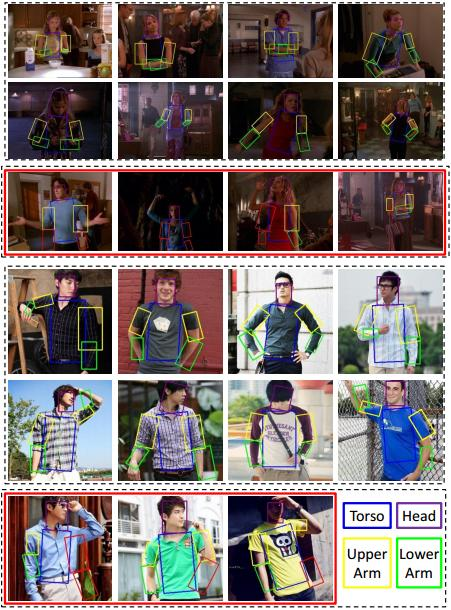
\includegraphics[width=.8\textwidth]{img/result.jpg}
\bicaption{\textbf{我们的算法在Buffy和DL数据集上得到的结果示例}
上面两个框中的结果是Buffy数据集上的,剩下的是DL数据集上的。
我们用带方向的矩形框来表示人体姿势识别的结果。
每个数据集对应的第一个框是正确的结果,而第二个框是错误的结果。
红色的矩形框代表错误的结果,其它颜色分别代表不同的人体躯干部位。}{\textbf{我们的算法在Buffy和DL数据集上得到的结果示例}
上面两个框中的结果是Buffy数据集上的,剩下的是DL数据集上的。
我们用带方向的矩形框来表示人体姿势识别的结果。
每个数据集对应的第一个框是正确的结果,而第二个框是错误的结果。
红色的矩形框代表错误的结果,其它颜色分别代表不同的人体躯干部位。}{Fig}{\textbf{Visualization of pose results produced by our algorithm on the Buffy and DL datasets.}
The top two panels are from Buffy and the others are from DL. We use the oriented bounding box to denote the pose estimation.
The first panel of each dataset are correct results, while the second panel are incorrect results.
The bounding box with red color denote the incorrect estimation.}
\label{fig:result}
\end{figure}

\section{本章小结}
在本章中,我们设计了大量的实验来验证我们提出的方法的可行性,特别是在加进了衣服属性变量以后,
人体姿势预测结果的提升效果。
从定性和定量的角度去对比了我们的工作和前人工作的性能差异,并且分析了我们工作的优势和不足。
同时,我们展示了我们工作的另一个输出结果,将不同照片按照相似的衣服属性聚集在了一起,
这样对于做衣服聚类工作是非常有效的,并且我们利用F1分值对聚类结果进行了评测。
大量实验证明,本文提出的隐变量衣服属性方法取得了目前精度最好的人体姿势预测结果。
